\chapter{Title Chapter One}
% TODO: edit all this file

\section{Title section}

Here we've done some examples of tables.

\subsection{Table One}
\begin{table}[h]
  \centering
  \begin{tabular}{|lllll|}
    \toprule
    A  & B  & C  & D  & E  \\
    \midrule
    A1 & B1 & C1 & D1 & E1 \\
    A2 & B2 & C2 & D2 & E2 \\
    A3 & B3 & C3 & D3 & E3 \\
    \bottomrule
  \end{tabular}
  \caption{Table One}
  \label{Tab:tableone}
\end{table}
First example of table \ref{Tab:tableone}.
\subsection{Table Two}

\begin{table}[ht]
  \centering
  \begin{tabular}{|l|c|r|}
    \hline
    Item 11 & Item 12 & Item 13 \\
    \hline
    Item 21 & Item 22 & Item 23 \\
    \hline
  \end{tabular}
  \caption{Table Two}
  \label{Tab:tabletwo}
\end{table}
Second example of table \ref{Tab:tableone}.
\lipsum[1-1]
\subsection{Table Three}

\begin{table}[!ht]
  \centering
  \label{tab:table3}
  \begin{tabular}{|c|c|c|}
    \hline
    \textbf{Value 1}                            & \textbf{Value 2} & \textbf{Value 3}    \\
    \hline
    $\alpha$                                    & $\beta$          & $\gamma$            \\
    \hline
    \multicolumn{2}{|c|}{\multirow{2}{*}{1234}} & a                                      \\
    \cline{3-3}
    \multicolumn{2}{|c|}{}                      & b                                      \\
    \hline
    3                                           & 23.113231        & \multirow{2}{*}{c~} \\
    \cline{1-2}
    4                                           & 25.113231        &                     \\
    \hline
  \end{tabular}
  \caption{Table three}
  \label{Tab:tablethree}
\end{table}
Third example of table \ref{Tab:tablethree}.
\lipsum[1-1].
\subsection{Table Four}
\begin{table}[!ht]
  \centering
  \begin{tabular}{|l|l|l|l|l|l|}
    \hline
    1  & Eldon Base        & 3   & 35    & Storage \& Organization        & 0.8  \\ \hline
    2  & 1.7 Cubic Foot    & 293 & 68.02 & Appliances                     & 0.58 \\ \hline
    3  & Cardinal Slant-D  & 293 & 2.99  & Binders and Binder Accessories & 0.39 \\ \hline
    4  & R380              & 483 & 3.99  & Telephones and Communication   & 0.58 \\ \hline
    5  & Holmes HEPA       & 515 & 5.94  & Appliances                     & 0.5  \\ \hline
    6  & G.E. Longer-Life  & 515 & 4.95  & Office Furnishings             & 0.37 \\ \hline
    7  & Angle-D Binderss  & 613 & 7.72  & Binders and Binder Accessories & 0.38 \\ \hline
    8  & SAFCO Mobile Desk & 613 & 6.22  & Storage \& Organization        & ~    \\ \hline
    9  & SAFCO Commercial  & 643 & 35    & Storage \& Organization        & ~    \\ \hline
    10 & Xerox 198         & 678 & 8.33  & Paper                          & 0.38 \\ \hline
  \end{tabular}
  \caption{Table Four}
  \label{Tab:tablefour}
\end{table}
Fourth example of table \ref{Tab:tablefour}.
\lipsum[1-1].
\section{Figure}
Here we've done some examples of Figure.

\subsection{Figure One}

\begin{figure}[!ht]
  
\includegraphics[width=\linewidth]{../images/fig1.png}
  \caption{Fig one}
  \label{fig:figone}
\end{figure}
First Example for figure  \ref{fig:figone}.
\lipsum[1-1]
\subsection{Figure Two}
\begin{figure}[!ht]
  \centering
  \begin{subfigure}[b]{0.4\linewidth}
    
\includegraphics[width=\linewidth]{../images/fig1.png}
    \caption{Fig a.}
  \end{subfigure}
  \begin{subfigure}[b]{0.4\linewidth}
    
\includegraphics[width=\linewidth]{../images/fig1.png}
    \caption{Fig b.}
  \end{subfigure}
  \caption{Figure two}
  \label{fig:figtwo}
\end{figure}
Second Example for figure  \ref{fig:figtwo}.
\lipsum[1-1]

\subsection{Figure Three}
Lorem ipsum dolor sit amet, consectetuer adipiscing elit. Ut purus elit, vestibulum
ut, placerat ac, adipiscing vitae, felis. Curabitur dictum gravida mauris \ref{fig:fig3}.

\begin{wrapfigure}{l}{0.25\textwidth}
  
\includegraphics[width=0.9\linewidth]{../images/fig1.png}
  \caption{Figure Three}
  \label{fig:fig3}
\end{wrapfigure}

\lipsum[1-1]
\subsection{Figure Four}

\begin{wrapfigure}{r}{0.4\textwidth} %this figure will be at the right
  \centering
  
\includegraphics[width=0.3\textwidth]{./images/fig1.png}
  \caption{Figure Four}
  \label{fig:fig4}
\end{wrapfigure}

\lipsum[1-1] \ref{fig:fig4}.

\subsection{Figure Five}

\begin{figure}[ht]
  \centering
  \begin{subfigure}{0.4\textwidth}
    
\includegraphics[width=\textwidth]{../images/fig1.png}
    \caption{First subfigure.}
    \label{fig:a-b-first}
  \end{subfigure}
  \hfill
  \begin{subfigure}{0.4\textwidth}
    
\includegraphics[width=\textwidth]{../images/fig1.png}
    \caption{Second subfigure.}
    \label{fig:a-b-second}
  \end{subfigure}
  \hfill
  \begin{subfigure}{0.4\textwidth}
    
\includegraphics[width=\textwidth]{../images/fig1.png}
    \caption{Third subfigure.}
    \label{fig:a-b-third}
  \end{subfigure}

  \caption{Creating subfigures in \LaTeX.}
  \label{fig:fig5}
\end{figure}
\lipsum[1-1] \ref{fig:fig5}.

\subsection{Figure Six}
\begin{figure}[ht]
  \begin{center}
    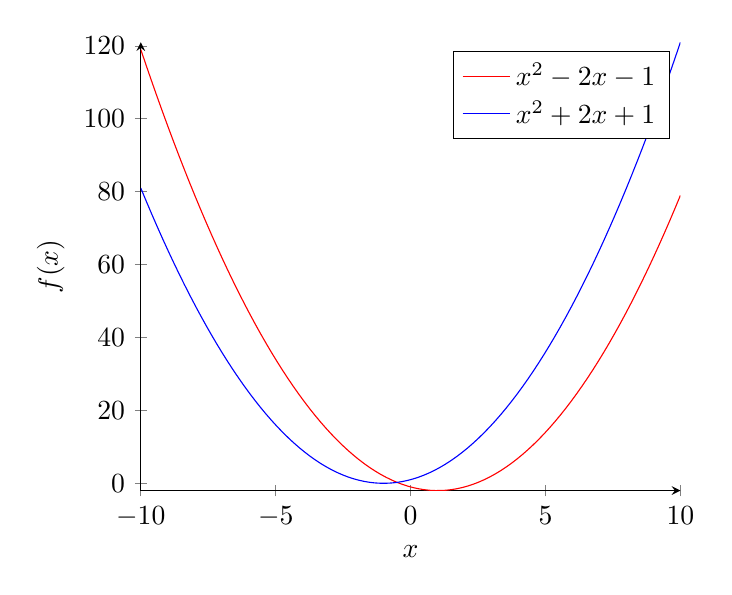
\begin{tikzpicture}
      \begin{axis}[
          axis lines = left,
          xlabel = \(x\),
          ylabel = {\(f(x)\)},
        ]
        \addplot [
          domain=-10:10,
          samples=100,
          color=red,
        ]
        {x^2 - 2*x - 1};
        \addlegendentry{\(x^2 - 2x - 1\)}
        \addplot [
          domain=-10:10,
          samples=100,
          color=blue,
        ]
        {x^2 + 2*x + 1};
        \addlegendentry{\(x^2 + 2x + 1\)}

      \end{axis}
    \end{tikzpicture}
    \caption{Plot.}
    \label{fig:fig6}
  \end{center}
\end{figure}
\lipsum[1-1] \ref{fig:fig6}.

\subsection{Figure Seven}
\begin{figure}[ht]
  \begin{center}
    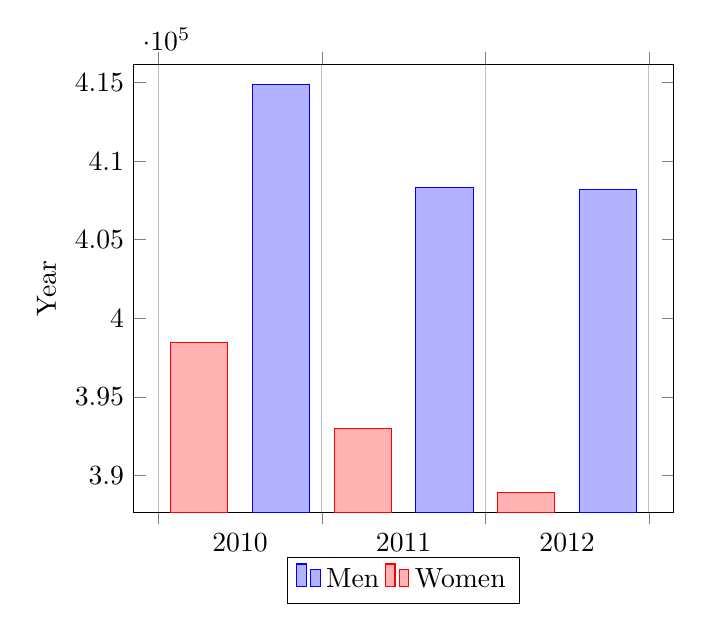
\begin{tikzpicture}
      \begin{axis}[
          x tick label style={
              /pgf/number format/1000 sep=},
          ylabel=Year,
          enlargelimits=0.05,
          legend style={at={(0.5,-0.1)},
              anchor=north,legend columns=-1},
          ybar interval=0.7,
        ]
        \addplot
        coordinates {(2012,408184) (2011,408348)
            (2010,414870) (2009,412156)};
        \addplot
        coordinates {(2012,388950) (2011,393007)
            (2010,398449) (2009,395972)};
        \legend{Men,Women}
      \end{axis}
    \end{tikzpicture}
    \caption{Plot 2.}
    \label{fig:fig7}
  \end{center}
\end{figure}
\lipsum[1-1] \ref{fig:fig7}.

\subsection{Figure Eight}
\begin{figure}[ht]
  \begin{center}
    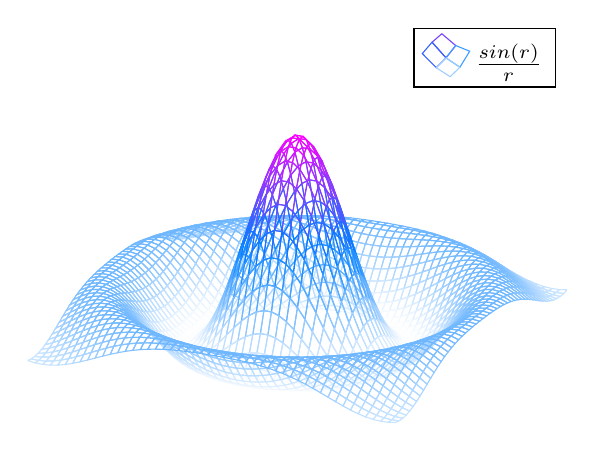
\begin{tikzpicture}
      \begin{axis}[
          hide axis,
          colormap/cool,
        ]
        \addplot3[
          mesh,
          samples=50,
          domain=-8:8,
        ]
        {sin(deg(sqrt(x^2+y^2)))/sqrt(x^2+y^2)};
        \addlegendentry{\(\frac{sin(r)}{r}\)}
      \end{axis}
    \end{tikzpicture}
    \caption{Plot 3.}
    \label{fig:fig8}
  \end{center}
\end{figure}
\lipsum[1-3] \ref{fig:fig8}.
